\documentclass{beamer}
\usefonttheme{professionalfonts}
\usepackage{amsmath}
\usepackage[linesnumbered,ruled,vlined]{algorithm2e}
\usepackage{tabularx}
\usepackage{makecell}
\usepackage{graphicx}
\usepackage{tikz}
\usepackage[absolute,overlay]{textpos}
\usepackage{pgfpages}

\graphicspath{{assets/}}
\setbeamertemplate{navigation symbols}{}
\setbeamerfont{caption}{size=\scriptsize}

\title[RNA ML Architecture Comparison]{\textbf{On the performance of machine learning architectures for RNA structure prediction}}
\subtitle{Bachelor thesis defense}
\author{Aaron Masur}
\date{July 13, 2026}


\newcommand{\smallcap}[1]{{\scriptsize\textbf{#1}}}
\newcommand{\takehome}[1]{\vspace{0.4em}\centering\Large $\Rightarrow$ \textbf{#1}}
\newcommand{\thesispicScale}{0.04}

% -----------------------------------------------------------------------------
% Editable chapter navigation bar
% Change these titles once you have your final structure.
\newcommand{\chapterone}{Research question intro}
\newcommand{\chaptertwo}{RNA basics}
\newcommand{\chapterthree}{Models I reviewed}
\newcommand{\chapterfour}{Pipeline}
\newcommand{\chapterfive}{Results}

% Set the active chapter before a frame with: \setchapternav{3}
% Hide/show the bar with: \showchapterbarfalse / \showchapterbartrue
\newif\ifshowchapterbar
\showchapterbarfalse
\newcommand{\currentchapter}{0}
\newcommand{\setchapternav}[1]{\renewcommand{\currentchapter}{#1}}

\newcommand{\chaptersegment}[2]{%
  \ifnum\currentchapter=#1
    \colorbox{blue!13}{\parbox[c][0.38cm][c]{0.185\paperwidth}{\centering\tiny\bfseries #1. #2}}%
  \else
    \colorbox{black!3}{\parbox[c][0.38cm][c]{0.185\paperwidth}{\centering\tiny\color{black!36} #1. #2}}%
  \fi
}

\setbeamertemplate{footline}{%
  \ifshowchapterbar
    {\setlength{\fboxsep}{0pt}%
    \hbox to \paperwidth{%
      \chaptersegment{1}{\chapterone}%
      \chaptersegment{2}{\chaptertwo}%
      \chaptersegment{3}{\chapterthree}%
      \chaptersegment{4}{\chapterfour}%
      \chaptersegment{5}{\chapterfive}%
      \makebox[0.075\paperwidth][c]{\tiny\color{black!45}\insertframenumber/\inserttotalframenumber}%
    }}%
  \fi
}

\begin{document}

% -----------------------------------------------------------------------------
{\setbeamertemplate{background canvas}{\begin{tikzpicture}[remember picture,overlay]
    \node[anchor=center,inner sep=0pt,opacity=0.15] at (current page.center) {
\includegraphics[width=\paperwidth,height=\paperheight,keepaspectratio]{rna_ensemble2.png}};
  \end{tikzpicture}}
\begin{frame}[plain]
  \titlepage
\end{frame}
\setbeamertemplate{background canvas}{}
}

% -----------------------------------------------------------------------------
\begin{frame}[plain]
\begin{tikzpicture}[remember picture,overlay]
    \node[anchor=center,inner sep=0pt,opacity=1] at (current page.center) {\includegraphics[width=\paperwidth,height=\paperheight,keepaspectratio]{thesisinpictures.png}};
  \end{tikzpicture}
\end{frame}

% -----------------------------------------------------------------------------
{\setbeamertemplate{background canvas}{\begin{tikzpicture}[remember picture,overlay]
    \node[anchor=center,inner sep=0pt,opacity=0.35] at (current page.center) {\includegraphics[width=\paperwidth,height=\paperheight,keepaspectratio]{thesisinpictures.png}};
  \end{tikzpicture}}
\begin{frame}{Overview}
  \vfill
  \begin{enumerate}
    \large
    \item<1-> \chapterone
    \item<2-> \chaptertwo
    \item<3-> \chapterthree
    \item<4-> \chapterfour
    \item<5-> \chapterfive
  \end{enumerate}
  \vfill
  \note{This is intentionally only a rough map. The chapter titles are defined once in the preamble, so they can be changed later. After this slide, the same structure appears as a small navigation strip at the bottom of each slide.}
\end{frame}
\setbeamertemplate{background canvas}{}
}

\showchapterbartrue
\setchapternav{1}

% -----------------------------------------------------------------------------
\begin{frame}{The question behind the thesis}
  \vfill
  \begin{minipage}{0.47\textwidth}
    \centering
    
\includegraphics[width=\linewidth,keepaspectratio]{rna_representations.png}\\[3pt]
    \footnotesize RNA structure as something we can compute with
  \end{minipage}\hfill
  \begin{minipage}{0.49\textwidth}
    \large
    Many modern RNA folding tools report strong scores.\\[0.7em]
    But those tools often combine neural networks with \textbf{constraints}, \textbf{preprocessing}, \textbf{postprocessing}, and \textbf{dataset effects}.\\[0.7em]
    \textbf{So what can the architecture itself learn?}
  \end{minipage}
  \vfill
  \note{Start chill: This thesis is not about building the next state-of-the-art RNAfold replacement. It is about isolating three architecture types and asking how much of the folding signal they can learn under comparable, deliberately simplified conditions.}
\end{frame}

% -----------------------------------------------------------------------------
\begin{frame}{Two research questions}
  \vfill
  \begin{enumerate}
    \item<1-> \textbf{How much data is necessary} for FFN, CNN, and BLSTM models to perform sufficiently well?
          \vspace{1em}
    \item<2-> \textbf{How do these architectures behave on biased datasets} such as base-pair span, GC content, helix length, and multiloops?
  \end{enumerate}
  \vfill
  \only<3->{\takehome{Not just ``which model wins'', but what each architecture learns.}}
  \note{Mention that RQ1 is about data scaling and the basic ability to learn RNA folding patterns. RQ2 is about stress testing: if I bias the training data in a controlled way, does the model still generalize or does it rely on that bias?}
\end{frame}

% -----------------------------------------------------------------------------
\setchapternav{2}
\begin{frame}{What is RNA?}
  \begin{minipage}{0.50\textwidth}
    
\includegraphics[width=\linewidth,keepaspectratio]{rna_ensemble.png}
  \end{minipage}\hfill
  \begin{minipage}{0.47\textwidth}
    \large
    RNA is a sequence over\\[-2pt]
    \[\{A,C,G,U\}\]
    It folds by forming base pairs.\\[0.6em]
    The relevant abstraction in this thesis is the \textbf{secondary structure}: which positions pair with which other positions.
  \end{minipage}
  \note{Explain RNA very briefly: It is not only messenger RNA; many RNAs have functions that depend on their shape. The central idea is ``form defines function''. This thesis focuses on secondary structure because it is computationally tractable and already contains a lot of structural information.}
\end{frame}

% -----------------------------------------------------------------------------
\begin{frame}{RNA secondary structure has rules}
  \centering
  
\includegraphics[width=0.86\textwidth,height=0.70\textheight,keepaspectratio]{rna_constraints.png}
  \vspace{0.3em}

  \small canonical pairs, minimum loop length, one partner per base, no pseudoknots
  \note{Use the picture. Valid structure top left; the other examples show why the task is not just arbitrary binary classification. There are biochemical and structural constraints. These are exactly the kinds of rules plain networks would need to learn if we do not hard-code them.}
\end{frame}

% -----------------------------------------------------------------------------
\begin{frame}{From sequence to base-pair matrix}
  \begin{minipage}{0.56\textwidth}
    \centering
    
\includegraphics[width=\linewidth,keepaspectratio]{rna_representations.png}
  \end{minipage}\hfill
  \begin{minipage}{0.40\textwidth}
    \large
    A base-pair matrix is an $L\times L$ image-like representation.\\[0.7em]
    Cell $(i,j)$ says how likely base $i$ pairs with base $j$.\\[0.7em]
    This makes RNA folding look like a sparse matrix prediction problem.
  \end{minipage}
  \note{Point to the dot plot / base-pair matrix. In the thesis the network output is a matrix of scores/logits, later converted to probabilities and thresholded. Important: the matrix is sparse because each base can pair with at most one other base.}
\end{frame}

% -----------------------------------------------------------------------------
\begin{frame}{The baseline target: RNAfold / Zuker-style folding}
  \vfill
  \begin{minipage}{0.50\textwidth}
    \Large
    Classical folding: find a structure with low free energy.\\[1em]
    \[p(s)=\frac{1}{Z}\,e^{-E(s)/(kT)}\]
  \end{minipage}\hfill
  \begin{minipage}{0.46\textwidth}
    \large
    In this thesis, synthetic sequences are generated and their target structures are produced by \textbf{ViennaRNA RNAfold}.\\[0.7em]
    So the networks are trained to approximate this biochemical model.
  \end{minipage}
  \vfill
  \note{This is the bridge from biology to ML. I am not claiming the synthetic labels are experimentally verified reality. The goal is controlled: can the architecture learn the folding mechanism represented by RNAfold?}
\end{frame}

% -----------------------------------------------------------------------------
\setchapternav{3}
\begin{frame}{The three modeling principles}
  \vfill
  \begin{minipage}{0.32\textwidth}
    \centering
    
\includegraphics[width=\linewidth,keepaspectratio]{ffn_basic.png}\\[3pt]
    \smallcap{FFN}\par
    \footnotesize fully connected feature integration
  \end{minipage}\hfill
  \begin{minipage}{0.32\textwidth}
    \centering
    
\includegraphics[width=\linewidth,keepaspectratio]{cnn_convolution.png}\\[3pt]
    \smallcap{CNN}\par
    \footnotesize local pattern extraction
  \end{minipage}\hfill
  \begin{minipage}{0.32\textwidth}
    \centering
    
\includegraphics[width=\linewidth,keepaspectratio]{lstm_cell.png}\\[3pt]
    \smallcap{BLSTM}\par
    \footnotesize sequential dependency modeling
  \end{minipage}
  \vfill
  \note{Use this as the architecture overview. FFN: everything connected, but no explicit locality or sequence order bias. CNN: kernels scan for local motifs and reuse weights, very natural for matrix-like structure. BLSTM: processes sequence left-to-right and right-to-left, so long-range sequential context should in principle matter.}
\end{frame}

% -----------------------------------------------------------------------------
\begin{frame}{FFN: fully connected, but no structural prior}
  \centering
  
\includegraphics[width=0.78\textwidth,height=0.62\textheight,keepaspectratio]{ffn_impl.png}
  \vfill
  \small one-hot encoded sequence $\rightarrow$ hidden layers $\rightarrow L^2$ output neurons
  \note{Explain that the FFN receives the fixed-length one-hot sequence and directly outputs the entire base-pair matrix. It has access to all positions, but it does not know that neighboring positions or symmetric matrix cells are special unless it learns this from data. This will matter later for the average-picture result.}
\end{frame}

% -----------------------------------------------------------------------------
\begin{frame}{CNN: local kernels on sequence and pairwise space}
  \begin{minipage}{0.52\textwidth}
    
\includegraphics[width=\linewidth,keepaspectratio]{cnn_convolution.png}
  \end{minipage}\hfill
  \begin{minipage}{0.44\textwidth}
    \large
    Kernels learn reusable local patterns.\\[0.8em]
    For RNA this suggests a bias towards motifs like stems, hairpins, and local constraints.\\[0.8em]
    High capacity: about 5 million trainable parameters in the optimized model.
  \end{minipage}
  \note{Stress the architectural hypothesis: CNNs should be strong on local spatial patterns and image-like base-pair matrices. That makes it plausible that they learn minimal loop length and local stem/helix patterns early. But high capacity also makes overfitting likely.}
\end{frame}

% -----------------------------------------------------------------------------
\begin{frame}{BLSTM: sequence context in both directions}
  \begin{minipage}{0.48\textwidth}
    
\includegraphics[width=\linewidth,keepaspectratio]{lstm_cell.png}
  \end{minipage}\hfill
  \begin{minipage}{0.48\textwidth}
    \large
    A BLSTM reads the RNA from both directions.\\[0.8em]
    Each nucleotide representation can contain left and right sequence context.\\[0.8em]
    The pair score is then computed from two position representations.
  \end{minipage}
  \note{This architecture is interesting because base pairs can be long-range. A BLSTM might encode information across the whole sequence. But it may be less naturally suited to very local geometric constraints like minimum loop length.}
\end{frame}

% -----------------------------------------------------------------------------
\setchapternav{4}
\begin{frame}{Design constraints I chose deliberately}
  \vfill
  \begin{minipage}{0.31\textwidth}
    \centering
    \Huge $\circledast$\\[-2pt]
    \normalsize synthetic data\\[3pt]
    \footnotesize controlled biases, RNAfold labels
  \end{minipage}\hfill
  \begin{minipage}{0.31\textwidth}
    \centering
    \Huge $100$\\[-2pt]
    \normalsize fixed length\\[3pt]
    \footnotesize fair FFN comparison, no padding effects
  \end{minipage}\hfill
  \begin{minipage}{0.31\textwidth}
    \centering
    \Huge $\varnothing$\\[-2pt]
    \normalsize no dropout / weight decay\\[3pt]
    \footnotesize expose architecture behavior
  \end{minipage}
  \vfill
  \note{This is important to say defensively. These are limitations, but they are also design decisions. Synthetic data lets me control structure and sequence bias. Fixed length keeps the FFN comparable. No regularization makes overfitting visible as part of the architecture behavior instead of hiding it.}
\end{frame}

% -----------------------------------------------------------------------------
\begin{frame}{Pipeline: from data to evaluation}
  \centering
  \vspace{0.7em}
  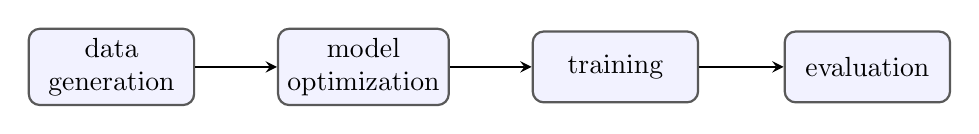
\begin{tikzpicture}[node distance=1.3cm, >=stealth, thick]
    \tikzstyle{box}=[draw=black!65, fill=blue!5, rounded corners=4pt, minimum width=2.1cm, minimum height=0.9cm, align=center]
    \node[box] (d) {data\\generation};
    \node[box, right of=d, xshift=1.9cm] (o) {model\\optimization};
    \node[box, right of=o, xshift=1.9cm] (t) {training};
    \node[box, right of=t, xshift=1.9cm] (e) {evaluation};
    \draw[->] (d) -- (o);
    \draw[->] (o) -- (t);
    \draw[->] (t) -- (e);
  \end{tikzpicture}
  \vfill
  \begin{minipage}{0.72\textwidth}
    \large
    The framework was written in Python/PyTorch and keeps the experimental loop identical across architectures.
  \end{minipage}
  \vfill
  \note{Walk through this slowly. Data generation: synthetic sequence and RNAfold label. Optimization: tune architecture and non-architecture hyperparameters such as threshold and positive class weight. Training: BCEWithLogitsLoss plus Adam, early stopping on validation MCC. Evaluation: independent test set, MCC and RNA-specific metrics.}
\end{frame}

% -----------------------------------------------------------------------------
\setchapternav{5}
\begin{frame}{RQ1 setup: how much data is enough?}
  \vfill
  \begin{center}
    \renewcommand{\arraystretch}{1.28}
    \begin{tabular}{c|c|c|c|c|c}
      \textbf{train size} & 200  & 1,000 & 5,000    & 10,000 & 50,000  \\
      \hline
      \textbf{idea}       & tiny & small & moderate & large  & scaling
    \end{tabular}
  \end{center}
  \vspace{1em}
  \large
  Each optimized architecture is trained on each size and evaluated on an independent 10,000-sequence test set.\\[0.6em]
  Primary score: \textbf{MCC}. Additional RNA metrics: symmetry, sparsity, non-canonical ratio, minimum loop length.
  \note{Mention that MCC is useful because base-pair matrices are very imbalanced: almost all cells are zeros. Accuracy would be misleading. The extra RNA metrics explain what the model learned structurally, not just whether the MCC went up.}
\end{frame}

% -----------------------------------------------------------------------------
\begin{frame}{RQ1 result: MCC scaling}
  \centering
  \renewcommand{\arraystretch}{1.25}
  \begin{tabular}{c|ccccc}
    \textbf{Model} & \textbf{200} & \textbf{1,000} & \textbf{5,000} & \textbf{10,000} & \textbf{50,000} \\
    \hline
    FFN            & 0.0104       & 0.0184         & 0.0257         & 0.0272          & 0.0280          \\
    CNN            & 0.2711       & 0.3165         & 0.3997         & 0.3976          & 0.4260          \\
    BLSTM          & 0.0000       & 0.0000         & 0.2924         & 0.3043          & 0.3359          \\
  \end{tabular}
  \vfill
  \only<2->{\takehome{CNN works early; BLSTM needs roughly 5,000; FFN stays near zero.}}
  \note{This is one of the central slides. Say: FFN is basically not solving the task. CNN already gets a meaningful MCC at 200 and improves with data. BLSTM is flat at zero for 200 and 1000 because predictions are below its optimized threshold; after 5000 it starts producing meaningful structures.}
\end{frame}

% -----------------------------------------------------------------------------
\begin{frame}{RQ1 visual result: what the models predict}
  \centering
  
\includegraphics[width=0.82\textwidth,height=0.73\textheight,keepaspectratio]{rq1_bpm_table.png}
  \note{Use the picture more than the numbers. FFN forms a broad average-looking pattern with many false positives, rather than sequence-specific folding. CNN predictions are sparse and already close to real base-pair diagonals. BLSTM with little data is too diffuse or below threshold, then begins to show structure from 5000 onward.}
\end{frame}

% -----------------------------------------------------------------------------
\begin{frame}{RQ1 RNA metrics: low vs. high data}
  \vfill
  \begin{minipage}{0.49\textwidth}
    \centering
    
\includegraphics[width=\linewidth,keepaspectratio]{rq1_metrics_200.png}\\[3pt]
    \footnotesize train size 200
  \end{minipage}\hfill
  \begin{minipage}{0.49\textwidth}
    \centering
    
\includegraphics[width=\linewidth,keepaspectratio]{rq1_metrics_50000.png}\\[3pt]
    \footnotesize train size 50,000
  \end{minipage}
  \vfill
  \note{The exact curves are not something the audience must memorize. Main story: CNN learns RNA constraints surprisingly early, but overfits. BLSTM becomes useful only with more data and still does not learn minimum loop length. FFN's curves reflect a learned average matrix rather than RNA-specific folding.}
\end{frame}

% -----------------------------------------------------------------------------
\begin{frame}{RQ1 interpretation by architecture}
  \vfill
  \begin{tabularx}{\textwidth}{@{}>{\bfseries}l X@{}}
    FFN   & learned an average base-pair distribution, not a sequence-specific folding rule                   \\[0.9em]
    CNN   & strong with little data, good local constraints, but clear overfitting                            \\[0.9em]
    BLSTM & no useful thresholded predictions for 200/1,000; starts around 5,000; weak on minimum loop length \\
  \end{tabularx}
  \vfill
  \takehome{Architecture bias explains a lot of the behavior.}
  \note{This slide maps observations to the architectural hypotheses: FFN has no locality or sequence prior. CNN has local kernels, so it is strong on local motifs and constraints. BLSTM has sequence context and lower parameter count, so it generalizes differently, but it is not naturally forced to respect local matrix constraints.}
\end{frame}

% -----------------------------------------------------------------------------
\begin{frame}{RQ2 setup: biased datasets}
  \begin{minipage}{0.43\textwidth}
    \centering
    
\includegraphics[height=0.78\textheight,keepaspectratio]{rq2_avg_structures.png}
  \end{minipage}\hfill
  \begin{minipage}{0.53\textwidth}
    \large
    Models were trained and evaluated across controlled biases:\\[0.7em]
    \begin{itemize}
      \item base-pair span
      \item GC content
      \item helix length
      \item multiloop topology
    \end{itemize}
  \end{minipage}
  \note{Explain that RQ2 is a transfer setup. Train on one biased dataset, evaluate on all datasets in the same experiment. This makes it possible to see whether a model learned a general rule or mostly adapted to the training distribution.}
\end{frame}

% -----------------------------------------------------------------------------
\begin{frame}{RQ2: base-pair span and GC content}
  \centering
  
\includegraphics[width=0.88\textwidth,height=0.76\textheight,keepaspectratio]{rq2_bp_gc_tables.png}
  \note{Talk through patterns, not every number. Base-pair span: CNN and BLSTM both suffer when train and eval span distributions differ, but BLSTM is especially sensitive to span shifts. GC content: performance drops towards extreme mismatches, especially for BLSTM. FFN remains low and mainly reflects average matrix similarity.}
\end{frame}

% -----------------------------------------------------------------------------
\begin{frame}{RQ2: helix length and multiloops}
  \centering
  
\includegraphics[width=0.86\textwidth,height=0.76\textheight,keepaspectratio]{rq2_hl_multi_tables.png}
  \note{Helix length is where the CNN sensitivity is most visible. The hypothesis is that kernels learn local helix motifs; if the helix-length distribution shifts, those patterns transfer less well. Multiloop shifts look less dramatic in MCC. Important caveat: MCC compares base-pair matrix cells and may not be a good metric for higher-order topology such as multiloop branch structure.}
\end{frame}

% -----------------------------------------------------------------------------
\begin{frame}{RQ2 interpretation}
  \vfill
  \begin{tabularx}{\textwidth}{@{}>{\bfseries}l X@{}}
    FFN        & mostly follows the average picture of train vs. evaluation set           \\[0.9em]
    BLSTM      & more sensitive to base-pair span and GC-content shifts                   \\[0.9em]
    CNN        & more sensitive to helix-length bias, likely due to kernel-learned motifs \\[0.9em]
    Multiloops & differences are moderate; MCC may hide topology errors                   \\
  \end{tabularx}
  \vfill
  \note{This slide should sound like the conclusion of RQ2. The sensitivities are not random; they can be explained from the architecture. FFN averages, CNN kernels, BLSTM sequential propagation. For multiloops, the result is also a metric lesson.}
\end{frame}

% -----------------------------------------------------------------------------
\begin{frame}{Overall take-home}
  \vfill
  \Large
  Plain architectures alone do \textbf{not} reach engineered RNA folding tools.\\[0.9em]
  But they reveal characteristic strengths and failure modes.\\[1.1em]
  \begin{center}
    \begin{tabular}{c|c}
      \textbf{Architecture} & \textbf{main lesson}            \\
      \hline
      FFN                   & learns dataset average          \\
      CNN                   & good local motifs, overfits     \\
      BLSTM                 & needs more data, global context \\
    \end{tabular}
  \end{center}
  \vfill
  \note{Connect back to the motivation: high performance of modern tools probably depends substantially on constraints, postprocessing, and specialized/hybrid designs. Architecture matters, but architecture alone is not enough here.}
\end{frame}

% -----------------------------------------------------------------------------
\begin{frame}{Outlook}
  \vfill
  \begin{minipage}{0.48\textwidth}
    \large
    \begin{itemize}
      \item hybrid architectures
      \item equal parameter-count comparison
      \item multiple random seeds
      \item finer bias sweeps
    \end{itemize}
  \end{minipage}\hfill
  \begin{minipage}{0.48\textwidth}
    \large
    \begin{itemize}
      \item real biological RNA datasets
      \item variable-length sequences
      \item transformers / graph neural networks
      \item topology-aware multiloop metrics
    \end{itemize}
  \end{minipage}
  \vfill
  \note{This is where you can say what you would do with more time. Especially emphasize hybrid architectures, because the results suggest complementary strengths. Also equal model complexity is important because the CNN had many more parameters than the BLSTM.}
\end{frame}

% -----------------------------------------------------------------------------
\begin{frame}{Danke für die Aufmerksamkeit!}
  \begin{center}
    \vfill
    \Huge Questions?
    \vfill
    
\includegraphics[width=0.64\textwidth,keepaspectratio]{rna_ensemble.png}
    \vfill
  \end{center}
  \note{End relaxed. If asked about limitations, answer honestly: synthetic labels, fixed length, no regularization, limited architectures, and MCC limitations. Then explain why each was chosen.}
\end{frame}

\end{document}
